\subsubsection{Studio di fattibilità}
In seguito alla pubblicazione dei capitolati d'appalto, il \textit{Responsabile di Progetto} avrà il compito di convocare una riunione per discutere sugli aspetti positivi e negativi dei capitolati. Sarà compito degli \textit{Analisti} redigere lo \textit{Studio di Fattibilità} in base a quanto emerso dalle riunioni.

\subsubsection{Analisi dei requisiti}
E' compito degli \textit{Analisti} stilare il documento \textit{Analisi dei Requisiti}.
In questo documento dovranno essere presenti tutti i requisiti ed i \gls{casi d'uso} emersi dall'analisi del capitolato e dalle riunioni con il Proponente.\\

\newpage
\paragraph{Requisiti}

I requisiti dovranno essere classificati per tipo e priorità, utilizzando la seguente notazione:

\begin{center}
	\begin{math}
		R \left [ importanza \right ] \left [ tipo\right ]\left [codice\right ]
	\end{math}
\end{center}
\begin{itemize}
	\item \textit{Importanza} può assumere i seguenti valori:
	\begin{itemize}
		\item \textbf{OBB:} Requisito obbligatorio;
		\item \textbf{DES:} Requisito desiderabile;
		\item \textbf{OPZ:} Requisito opzionale.
	\end{itemize}
	\item \textit{Tipo} può assumere i seguenti valori:
	\begin{itemize}
		\item \textbf{F:} Requisito funzionale;
		\item \textbf{Q:} Requisito di qualità;
		\item \textbf{P:} Requisito di prestazione;
		\item \textbf{V:} Requisito di vincolo.
	\end{itemize}
	\item \textit{Codice} rappresenta il codice univoco di ogni requisito in forma gerarchica.
\end{itemize}
Ogni requisito dovrà essere inserito (nel documento \textit{Analisi dei Requisiti}) in una tabella contenente il codice identificativo, una breve descrizione e la fonte.

\paragraph{Casi d'uso}
Dopo la stesura dei requisiti è sempre compito degli \textit{Analisti} analizzare i \gls{casi d'uso} (abbreviati con UC, Use Case).
Per ogni caso d'uso sono richieste le seguenti informazioni:
\begin{itemize}
	\item \textbf{Attori:} gli attori coinvolti nel caso d'uso (principali e secondari);
	\item \textbf{Scopo e descrizione:} una breve descrizione chiara e dettagliata del caso d'uso;
	%\item Codice identificativo: nel formato UCxx, dove xx indica un numero identificativo del caso d'uso;
	%\item Titolo: titolo sintetico del caso d'uso;
	\item \textbf{Precondizione:} la precondizione del requisito;
	\item \textbf{Flusso degli eventi:} specificare per ogni evento: descrizione, attori coinvolti e se lo scenario è descritto in dettaglio da un altro caso d'uso;
	%\item Diagramma: dovrà essere usato \gls{UML} 2.4 per la creazione dei diagrammi dei \gls{casi d'uso};
	\item \textbf{Postcondizione:} la postcondizione del requisito.
\end{itemize}

\newpage
\paragraph{Tracciamento dei requisiti}
Per il tracciamento dei requisiti è stato creato un \gls{database} che tiene traccia dei requisiti, \gls{casi d'uso} e tutte le dipendenze.
È stato realizzato un \gls{plugin} per il Content Management System (\gls{CMS}) \gls{WordPress} per renderne possibile il popolamento e l'interrogazione.
Il \gls{plugin} genera automaticamente il codice \LaTeX\ per l'\textit{Analisi dei Requisiti}.
Per sua natura, il \gls{plugin} è portabile su tutte le versioni di \gls{WordPress} ed alla fine del progetto sarà reso open-source in modo che possa essere riutilizzato da chi lo desideri. È stato scelto questo \gls{CMS} poiché, essendo conosciuto da due membri del gruppo, permette di concentrarsi esclusivamente sulla gestione dei requisiti tralasciando tutti gli aspetti di contorno, comprimendo così notevolmente i tempi di sviluppo.
\begin{figure}[h]
	\centering
	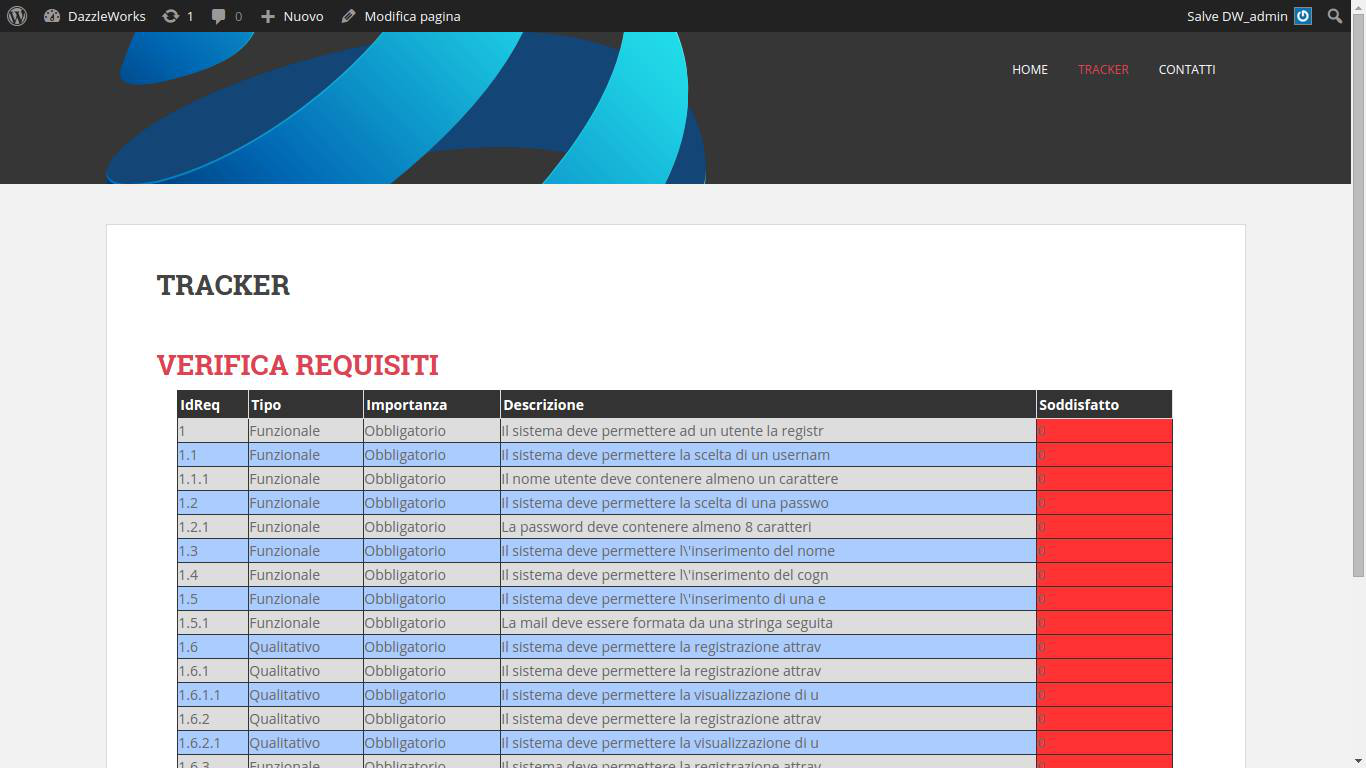
\includegraphics[width=0.7\linewidth]{img/tracker1}
	\caption[Pagina riepilogo requisiti]{Pagina riepilogo requisiti}
	\label{fig:tracker1}
\end{figure}
\begin{figure}[h]
	\centering
	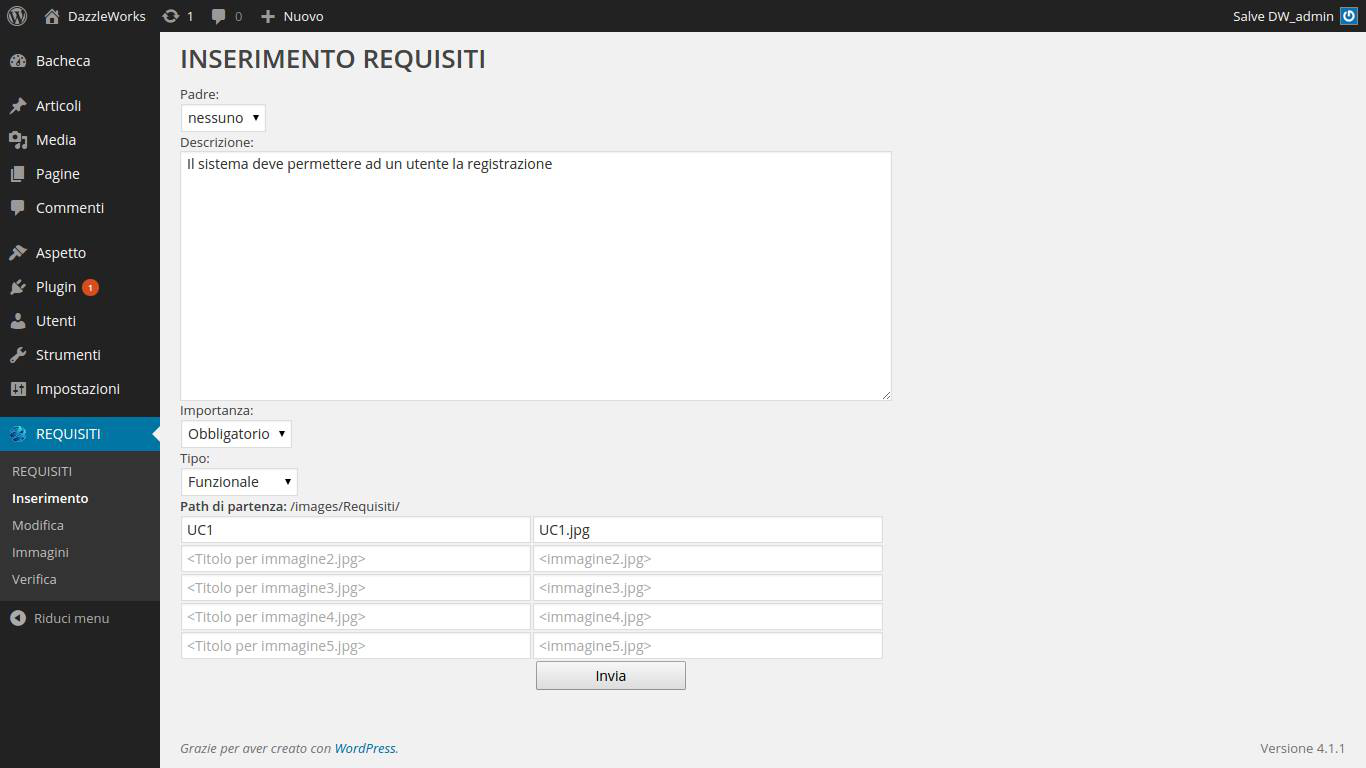
\includegraphics[width=0.7\linewidth]{img/tracker2}
	\caption[Pagina inserimento requisito]{Pagina inserimento requisito}
	\label{fig:tracker2}
\end{figure}

